\section{Deviations from the pre-specified plan}\label{app:deviations}
Deviations D1--D4 were decided before any model had been trained; at that point only the preprocessing log had been
inspected. D5 was decided after the subject-level models had been evaluated but before any result of the affected
(Riemannian) models existed.

\begin{enumerate}
  \item[D1] \textbf{Bad-channel detector.}
        \begin{itemize}
          \item \emph{Problem:} the pre-specified rule (flat signal, robust log-SD $z>5$, median neighbour correlation
                $<0.4$) flagged up to 48 of 129 channels in a recording. Of all flags, 94\% came from the
                neighbour-correlation criterion, and they included channels adjacent to the vertex reference with
                \emph{negative} neighbour correlations. Whole-recording correlation is not a valid quality measure on
                reference-dominated, artefact-laden data.
          \item \emph{Change:} the rule was replaced by the PREP implementation~\cite{bigdely2015prep}.
          \item \emph{Unchanged:} the 20\% exclusion threshold.
        \end{itemize}
  \item[D2] \textbf{Re-run.} Fourteen participants were re-run after an infrastructure failure: a library was being
        installed during the first run. Since D1 required a full re-run anyway, all 53 were re-processed.
  \item[D3] \textbf{Added model.} The ERP-covariance Riemannian model was added as a secondary model.
  \item[D4] \textbf{Added sensitivity analysis.} Exclusions affected \NExcludedMDD{} MDD and \NExcludedHC{} HC
        participants, so we added a sensitivity analysis of the primary model on all 53 participants.
  \item[D5] \textbf{Computational budget of the Riemannian models.}
        \begin{itemize}
          \item \emph{Problem:} timing one outer fold showed that the full protocol (10 repetitions plus 200
                permutations, i.e.\ 1{,}050 outer folds per model) would take more than 12~h, mostly because
                per-trial covariances were recomputed in every inner-loop fit.
          \item \emph{Change 1 (no effect on results):} for the tangent-space and MDM models, per-trial OAS
                covariances were computed once. Each covariance depends only on its own trial, so this involves no
                learning across samples; the tangent-space reference point, scaling, classifier and MDM centroids
                were still fitted inside each training fold. A unit test verifies identical predictions.
          \item \emph{Change 2:} the ERP-covariance model, whose class prototypes depend on labels and must be
                recomputed within each fold, used a fixed regularisation $C=0.1$ instead of an inner grid. A value
                fixed in advance cannot inflate performance; at worst it is slightly sub-optimal.
        \end{itemize}
  \item[D6] 	extbf{Post-hoc audit analyses (exploratory).} After all pre-specified results were known, an internal
        audit added the analyses of Sections~
ef{sec:audit-methods} and~
ef{sec:audit}. They do not replace,
        re-rank or re-threshold any pre-specified result. They are Holm-corrected among themselves and labelled
        exploratory throughout.
\end{enumerate}

\section{Preprocessing quality}
\begin{figure}[h]
\centering
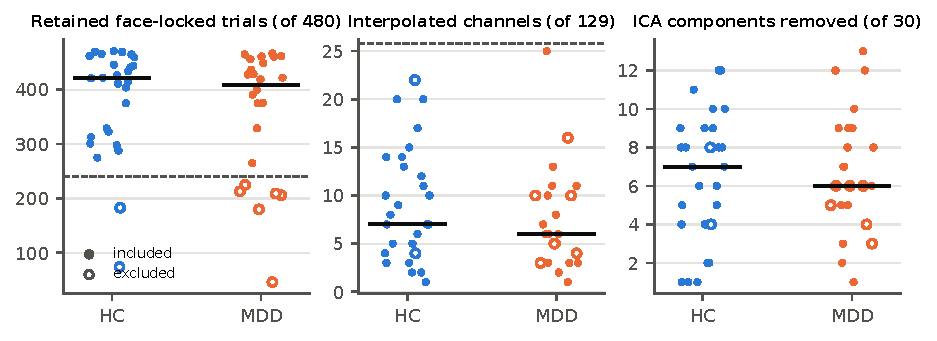
\includegraphics[width=\linewidth]{fig_quality}
\caption{Signal quality per participant: retained face-locked trials, interpolated channels and removed ICA
components. Open markers show participants excluded by the pre-specified criteria (dashed lines). Horizontal bars
are group medians.}
\label{fig:quality}
\end{figure}

\begin{figure}[h]
\centering
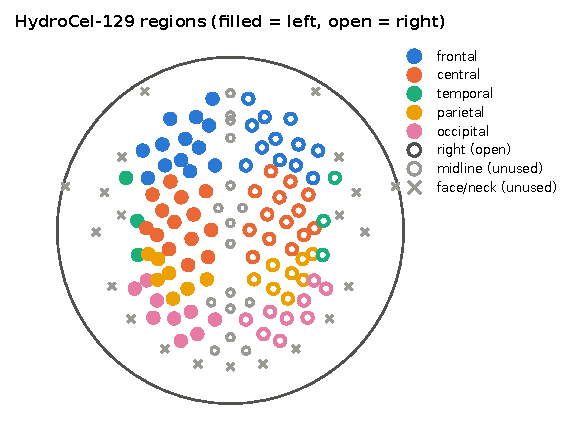
\includegraphics[width=0.55\linewidth]{fig_regions}
\caption{Assignment of HydroCel-129 electrodes to the ten regions, obtained by nearest 10--10 anchor on the fitted
head sphere. Filled markers are left-hemisphere electrodes and open markers right-hemisphere electrodes. Grey
electrodes (midline, and the face/neck ring more than \SI{115}{\degree} from the vertex) are not used for regional
features.}
\label{fig:regions}
\end{figure}

\section{Univariate group differences}
\begin{table}[h]
\centering\small
\caption{The ten features with the smallest uncorrected Mann--Whitney $p$ (MDD vs.\ HC, included participants).
$p_\text{FDR}$ is Benjamini--Hochberg corrected over all 288 features.}
\label{tab:uni}
\begin{tabular}{@{}llrrr@{}}
\toprule
Feature & Family & Cohen's $d$ & $p$ & $p_\text{FDR}$ \\
\midrule
\texttt{wpli\_theta\_central\_L\_\_temporal\_L} & connectivity & 1.38 & $<$0.001 & 0.04 \\
\texttt{sampen\_occipital\_L} & complexity & 0.79 & 0.003 & 0.45 \\
\texttt{rel\_lowgamma\_occipital\_L} & spectral & 0.57 & 0.005 & 0.47 \\
\texttt{sampen\_temporal\_R} & complexity & 0.76 & 0.009 & 0.62 \\
\texttt{rel\_beta\_occipital\_L} & spectral & 0.69 & 0.012 & 0.66 \\
\texttt{wpli\_beta\_central\_R\_\_occipital\_L} & connectivity & -0.70 & 0.018 & 0.66 \\
\texttt{sampen\_parietal\_L} & complexity & 0.72 & 0.020 & 0.66 \\
\texttt{lzc\_occipital\_L} & complexity & 0.71 & 0.022 & 0.66 \\
\texttt{lzc\_temporal\_R} & complexity & 0.72 & 0.022 & 0.66 \\
\texttt{pow\_lowgamma\_occipital\_L} & spectral & 0.64 & 0.024 & 0.66 \\
\bottomrule
\end{tabular}
\end{table}

\section{Feature dictionary}\label{app:dictionary}
Every subject-level feature is computed per participant without labels. Names join the family, the band or measure and the region with underscores, for example
\texttt{pow\_alpha\_frontal\_L}. Regions are frontal, central, temporal, parietal and occipital, each
left (L) or right (R).

\begin{table}[h]
\centering\scriptsize
\caption{The 288 pre-specified subject-level features.}
\label{tab:dictionary}
\begin{tabular}{@{}p{3.3cm}rp{9.2cm}@{}}
\toprule
Name pattern & $n$ & Definition and interpretation \\
\midrule
\texttt{pow\_<band>\_<region>} & 50 & $\log_{10}$ absolute Welch power (\si{\micro\volt\squared}) in delta 1--4, theta
  4--8, alpha 8--13, beta 13--30 and low gamma 30--40~Hz, averaged over the region's electrodes. Depends on skull
  thickness and impedance as well as on brain activity. \\
\texttt{rel\_<band>\_<region>} & 50 & Band power divided by 1--40~Hz power. Removes individual scale. The five
  bands of a region sum to $\approx0.94$, so they are nearly collinear. \\
\texttt{faa\_F3F4}, \texttt{faa\_F7F8} & 2 & Frontal alpha asymmetry, $\ln\alpha_R-\ln\alpha_L$ (E124/E24,
  E122/E33). Lower values mean relatively less left-frontal activity, which approach--withdrawal theory predicts in
  depression. \\
\texttt{erp\_<cond>\_n170L/R\_amp}, \texttt{\_lat} & 12 & Minimum amplitude and its latency at 140--200~ms, at
  clusters around P7/P8, per condition (fear, happy, sad). Structural face encoding. \\
\texttt{erp\_<cond>\_p300\_amp}, \texttt{\_lat} & 6 & Mean amplitude (250--500~ms) and peak latency at a
  centro-parietal cluster around Pz. Attentional allocation. \\
\texttt{erp\_<cond>\_lpp\_amp} & 3 & Mean amplitude at 400--600~ms, same cluster. Sustained motivated attention.
  Overlaps the P300 window ($r\approx0.9$ with P300 amplitude). \\
\texttt{wpli\_<band>\_<A>\_\_<B>} & 135 & Weighted phase-lag index between region-mean signals (45 pairs, theta,
  alpha and beta), multitaper over 2-s segments. It ignores zero-lag coupling, which reduces volume conduction. \\
\texttt{sampen\_<region>} & 10 & Sample entropy ($m=2$, $r=0.2$\,SD). Signal unpredictability. \\
\texttt{hfd\_<region>} & 10 & Higuchi fractal dimension ($k_\text{max}=10$). Signal roughness. \\
\texttt{lzc\_<region>} & 10 & Normalised Lempel--Ziv complexity of the median-binarised signal. \\
\bottomrule
\end{tabular}
\end{table}

Spectral, connectivity and complexity features are computed on the cleaned \emph{task} recording, not at rest.
Complexity and high-frequency power are sensitive to residual muscle activity (Section~\ref{sec:audit}).
